\chapter{Implementation}
\label{chap:implementation}

\section{Goals}

In Chapter \ref{chap:background} was discussed three main things:
\begin{itemize}
\item Workflow and environment
\item Advantages and disadvantages of static type checking
\item Available tools and alternatives
\end{itemize}

Let's clarify what tools will be used and what we would like to achieve using
them. It necessary to keep in mind that trade offs should be sufficient, for
example feedback cycle must remain short and existing workflow shouldn't be
broken.

First tool is clojure.spec. As mentioned in Chapter \ref{chap:background} it has
several important advantages, integrates with already existing tools and will be
part of languages in the next major release. Second tool is spectrum, which
allows to do static analysis of the code. Third is an IDE (Emacs+cider). Last
one is javacc-clojure parser, it written to assess metrics of the code for
deeper understanding of changes introduced by optional annotations.

Advantages of static type checking explained in Section
\ref{sec:statictypechecking} can be generalized and divided into three main
parts:

\begin{itemize}
\item Improved developer experience
\item Better communication
\item More robust software
\end{itemize}

On the other hand drawbacks of static type checking should be avoided when it
possible. Let's take a closer look at the points mentioned below in context of clojure.spec:

\textbf{Improved Developer Experience.} Error messages from macros are a
perennial challenge for new (and experienced) users of Clojure. Specs can be
used to conform data in macros instead of using a custom parser. And Clojure’s
macro expansion will automatically use specs, when present, to explain errors to
users. Moreover it can provide similar messages between different platforms
(jvm, clr, js). This should result in a greatly improved experience for users
when errors occur.

\textbf{Better Communication.} Clojure is a dynamic language, and thus far we have relied
on documentation or external libraries to explain the use and behavior of
functions and libraries. But documentation is difficult to produce, is
frequently not maintained, cannot be automatically checked and varies greatly in
quality. Specs are expressive and precise. Including spec in Clojure creates a
lingua franca with which we can state how our programs work and how to use them.

\textbf{More Robust Software.} Clojure has always been about simplifying the development
of robust software. In all languages, dynamic or not, tests are essential to
quality - too many critical properties are not captured by common type systems.
spec has been designed from the ground up to directly support generative testing
via test.check. When you use spec you get generative tests for free.

As an addition clojure.spec provides more power. A key advantage of
specifications over documentation is the leverage they provide. In particular,
specs can be utilized by programs in ways that docs cannot. Defining specs takes
effort, and spec aims to maximize the return you get from making that effort.
spec gives you tools for leveraging specs in documentation, validation, error
reporting, destructuring, instrumentation, test-data generation and generative
testing.

Taken together, the features of tools demonstrate the ongoing advantages of a
powerful dynamic language like Clojure for building robust software - superior
expressivity, instrumentation-enhanced REPL-driven development, sophisticated
testing and more flexible systems.

\section{Improved development experience}
This section shows how to achieve improved development experience and get
consistent error messages across different platforms.

Clojure 1.9 is in alpha state right now and there are probably no public
projects extensively using it, that is why all experiments will be conducted on
sample project. Source code provided in \ref{chap:appendix}. Let's start from
sum function example:

\subsection{Destructuring}

\begin{minted}{clojure}
(defn simple-sum
  "Just a sum function."
  [a b]
  (+ a b))
\end{minted}

Definition of the function is pretty straightforward, but in real world
functions can be slightly complex. Even in example below it is not obvious,
which types of arguments this function accepts and what it produces, but let's
clarify what arguments should be acceptable for this function by defining
\texttt{::num} spec.


\begin{minted}{clojure}
(s/def ::num (s/or :float float?
                   :int   integer?
                   :ratio ratio?))
;; => :dat.core/num
(s/def ::even-int (s/and even? integer?))
;; => :dat.core/even-int
\end{minted}

This code produces two specs with predicates composed via \texttt{s/or} and
\texttt{s/and}, which registered under \texttt{dat.core} namespace. After that
value can be validated using this spec. It is important to understand that it
provides two features: validation in the code for business logic and validation
of the code for robustness of the software product.

\begin{minted}{clojure}
(def good-numbers [0.21 1/7 42])
(def not-so-good-numbers [0.21 1/7 42 :keyword "str"])
(map #(s/valid? ::num %) not-so-good-numbers)
;; => (true true true false false)
(map #(s/valid? ::even-int %) not-so-good-numbers)
;; => (false false true false false)
\end{minted}

Nothing really special here, but let's take a look at more interesting example.
Spec can be registered, also specs can be in-place like in example below:

\begin{minted}{clojure}
(s/conform (s/coll-of ::num) good-numbers)
;; => [[:float 0.21] [:ratio 1/7] [:int 42]]
(s/conform (s/coll-of ::num) not-so-good-numbers)
;; => :clojure.spec/invalid
\end{minted}

\texttt{(s/coll-of ::num)} returns new spec as a result of function, but it is
also a great example of destructuring, it's not necessary to write additional
parser to convert your collection in more meaningful structure, it's enough to
define spec and just conform your data. It is pretty handy especially in
data-intensive applications.

\subsection{Better error messages}
\label{sec:bettererrormessages}
In the example above first conform went well, but the second produced
\texttt{:clojure.spec/invalid} keyword, but what the problem with it? Luckily,
it is easy to understand that using \texttt{s/explain} function:

\begin{minted}{clojure}
(s/explain ::even-int 0.21)
;; => "val: 0.21 fails spec: :dat.core/even-int predicate: integer?\n"

(s/explain ::even-int 5)
;; => "val: 5 fails spec: :dat.core/even-int predicate: even?\n"
\end{minted}

It looks like basic type errors in statically typed languages. It is good, but
according to reality compiler errors in many languages are very cryptic and hard
to understand. How clojure.spec would behave in more complex environment?

\begin{minted}{clojure}
(s/explain-data (s/coll-of ::num) not-so-good-numbers)

;; {:clojure.spec/problems
;;  ({:path [:float],
;;    :pred float?,
;;    :val :keyword,
;;    :via [:dat.core/num],
;;    :in [3]}
;;   {:path [:int],
;;    :pred integer?,
;;    :val :keyword,
;;    :via [:dat.core/num],
;;    :in [3]}
;;   {:path [:ratio],
;;    :pred ratio?,
;;    :val :keyword,
;;    :via [:dat.core/num],
;;    :in [3]}
;;   {:path [:float],
;;    :pred float?,
;;    :val "str",
;;    :via [:dat.core/num],
;;    :in [4]}
;;   {:path [:int],
;;    :pred integer?,
;;    :val "str",
;;    :via [:dat.core/num],
;;    :in [4]}
;;   {:path [:ratio],
;;    :pred ratio?,
;;    :val "str",
;;    :via [:dat.core/num],
;;    :in [4]})}
\end{minted}

Clojure.spec can generate error messages, but it also can generate data
structures, which contains paths of the problems. In this example it is clear
that values in \texttt{not-so-good-numbers} on position 3 and 4 are violates all
predicates in composed predicate. Resulting data structure is a list of
problems, each problem represented as a map with following keys:

\begin{itemize}
\item val - the value in the user’s input that does not match
\item spec - the spec that was being evaluated
\item at - a path (a vector of keywords) indicating the location within the spec where
the error occurred - the tags in the path correspond to any tagged part in a
spec (the alternatives in an or or alt, the parts of a cat, the keys in a map,
etc)
\item predicate - the actual predicate that was not satsified by val
\item in - the key path through a nested data val to the failing value. In this
example, the top-level value is the one that is failing so this is essentially
an empty path and is omitted.

\end{itemize}

This form of report very powerful, it not only helps developers to understand
source of problem, but also allows to deal with it programmatically, it
especially important for more complex case. In addition to it such data can be
easily visualized. Such way gives a tool for current problems and place for
future development.

\subsection{Sampling data}
\label{sec:samplingdata}
In world of programming it is very hard to give names to functions and
variables, but it also hard to come up with values for test, examples and so on,
but if we know type or even more complex predicate about data, why developers
should create sample data structures and fill them with values by hands?
Actually they don't, it is very easy to generate them from specs.

\begin{minted}{clojure}
(s/exercise ::num)
;; ([-2.0 [:float -2.0]]
;;  [-1 [:int -1]]
;;  [-2 [:int -2]]
;;  [1/2 [:ratio 1/2]]
;;  [1.0 [:float 1.0]]
;;  [1/2 [:ratio 1/2]]
;;  [8 [:int 8]]
;;  [-1 [:int -1]]
;;  [-5 [:int -5]]
;;  [7/4 [:ratio 7/4]])

(s/exercise ::even-int)
;; ([0 0]
;;  [0 0]
;;  [-4 -4]
;;  [-2 -2]
;;  [0 0]
;;  [-4 -4]
;;  [-2 -2]
;;  [0 0]
;;  [-508 -508]
;;  [1548 1548])
\end{minted}

Not only simple specs can be exercised, but more much complex. For some cases it
necessary to write specific generators, but for simple one generators provided
out of the box and works well. Moreover functions can be exercised too:

\begin{minted}{clojure}
(s/fdef simple-sum
        :args (s/cat :a ::num :b ::num)
        :ret ::num)

(s/exercise-fn `simple-sum)
;; ([(-2.0 -2.0) -4.0]
;;  [(2.0 0) 2.0]
;;  [(-2 -0.5) -2.5]
;;  [(-2 Infinity) Infinity]
;;  [(4/5 -0.625) 0.17500000000000004]
;;  [(-1 -0.5) -1.5]
;;  [(-0.5 -3/7) -0.9285714285714286]
;;  [(1/3 -1) -2/3]
;;  [(-1.0 9) 8.0]
;;  [(1.1953125 -1) 0.1953125])
\end{minted}

This example introduces new macros \texttt{s/fdef}, which will be explained
later, but in fact \texttt{s/exercise-fn} just generates data as in the previous
example, but using spec defined in \texttt{s/fdef} and passes it to function
\texttt{simple-sum}. Nothing special, but it very good basis for further steps,
like automated software testing. Information about more advanced data sampling
can be found in \cite{specific}.

\section{Better communcation}
\label{sec:bettercommunication}
Developers often use external libraries or colleague's modules or even just
their own old code, but for languages such Clojure or Python it is not obvious,
which functions accepts which values (types of values). Such information can be
placed in docstring, but the problem is that documentation is hard to maintain,
it can vary in quality, became outdated or even contradictory and it means that
it doesn't linked with code. Much better, when there are something built in
language like type annotations, right? Clojure.spec is enough for this needs.

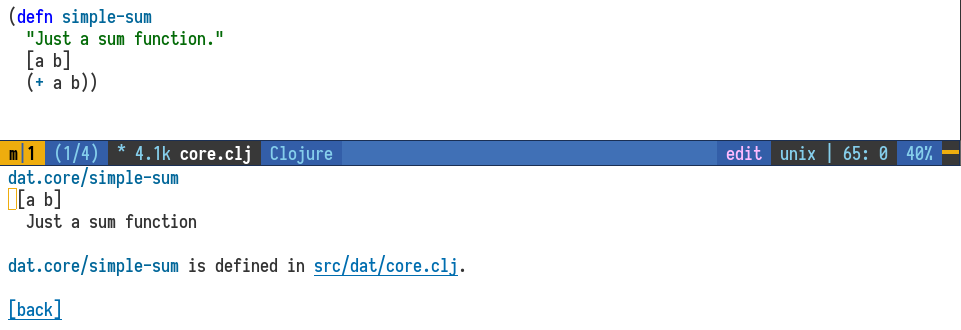
\includegraphics[width=\textwidth]{withoutspec}
% \subsection{Explanation}

Looking at documentation of function in dynamically typed language often doesn't
provide enough information and it is necessary to look at the source code, but
it is very time-consuming, especially when you need very small amount of
information about particular function.

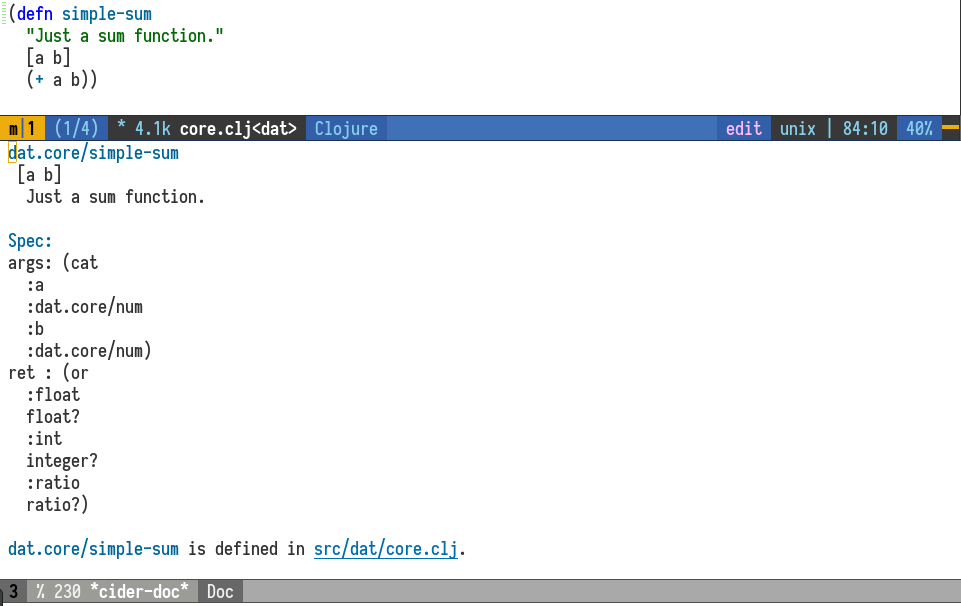
\includegraphics[width=\textwidth]{withspec}

Information about specs can be added to documentation in your IDE/repl, when
\texttt{s/fdef} macro is used. This macro defines which specs should be used for
arguments and return value, such information can be used later for sampling data
or generating documentation.

\begin{minted}{clojure}
(s/fdef simple-sum
        :args (s/cat :a ::num :b ::num)
        :ret ::num)
\end{minted}
This example provides very handy information about arguments and return value
``types'' for \texttt{simple-sum} function. Now, for developer it is not
necessary to investigate source code of the function to understand such simple
things as what parameters should be passed and what will be result of that
function. If it is not clear what mean particular spec it is easier to find its
definition and read it. Also, it is not necessary to place specs near the code,
they can be placed in separate files and namespaces as a documentation with
super cow powers.


\section{More robust software}

Let's take a look at more complex example extracted from real
commercial application. It is a part of generalized functions for REST API
testing and newcomers always has some troubles with that place. This code
simplified for thesis needs, but idea behind it is still actual.

\begin{minted}{clojure}
(def credentials
  {:admin   {:email "admin@test.io" :password "test#secret"}
   :manager {:email "manager@test.io" :password "test#secret"}
   :worker  {:email "worker@test.io" :password "test#secret"}
   :user    {:email "user@test.io" :password "test#secret"}})

(s/def ::user-type (-> credentials keys set))

(s/def ::token (s/and string?
                      #(< 6 (count %))))

(s/def ::real-token (s/and string?
                           #(< 6 (count %))
                           #(= "Token " (subs % 0 6))))

(s/def ::token-map (s/keys :req-un [::token]))

(defn get-token-for
  "Simple docstring here"
  [user-type]
  ;; somehow generate a token
  (case user-type
    :admin {:token "admin token"}
    :user {:token "user token"}
    {:token "Token default token"}))
\end{minted}


Initially, this code didn't have specs and someone used to come up with
question: What user-type is? After few similar questions
\texttt{credentials} map was created. It keys is a what we call user-type and
keys is a credentials of test users, which have this particular type. Now
everyone understand that user-type is one of the following keywords:
\texttt{:admin, :manager, :worker, :user}. It is a good illustration of a better
communcation using clojure.spec, but if we already use it what else can be done
with it?

\subsection{Static analysis}
Static analysis is possible, some huge projects like CircleCI used TypedClojure
for this needs, now when spec is in active development it is more rational to
use something more suitable for it. For example, Allen Rohner develop library
for static analysis using clojure.spec. Actually it is not very natural to do
static checking in Clojure, but it can be useful in pre-commit hooks or in
continuous integration scripts. Usage is pretty simple.

\begin{minted}{clojure}
(require '[spectrum.check :as check])

(check/check 'your.namespace)
;; flow-walk exception while walking:
;; file file:/home/abcdw/repos/typed-thesis/dat/src/dat/core.clj line 139 col 1
;;  (fn* ([user-type] (case user-type :admin {:token admin token}
;;  :user {:token user token} {:token Token default token})))
\end{minted}

This check will provide error messages like classic compiler with location in
the file and problem place, but it is not very suitable for live programming and
just a good addition, which can be done for free if project already uses
clojure.spec. Also, it is not so powerful as static analysis for languages with
static type systems because specs are optional, but it probably not worse than
other gradual type systems.

\subsection{Automated test generation}
First of all, to understand how function works in general and is it works at
all, the function can be exercised if it has specs related to it and see what
values will be produced. Pretty the same as in Section \ref{sec:samplingdata}.

\begin{minted}{clojure}
(fdef get-token-for
      :args (s/cat :user-type ::user-type)
      :ret ::token-map)

(s/exercise-fn `get-token-for)
;; ([(:admin) {:token "admin token"}]
;;  [(:user) {:token "user token"}]
;;  [(:user) {:token "user token"}]
;;  [(:user) {:token "user token"}]
;;  [(:admin) {:token "admin token"}]
;;  [(:admin) {:token "admin token"}]
;;  [(:admin) {:token "admin token"}]
;;  [(:manager) {:token "Token default token"}]
;;  [(:user) {:token "user token"}]
;;  [(:user) {:token "user token"}])
\end{minted}

It works well and from samples generated above it is obvious, but how to make
sure that it will work in the future, when some changes will be added. Obvious
solutions is to write a test using generated data, but what if specs will be
changed in the future? Data will become invalid. Second solution is to generate
data on each test execution. Do it using spec.test pretty easy:

\begin{minted}{clojure}
(stest/check `get-token-for)
;; ({:spec
;;   #object[clojure.spec$fspec_impl$reify__21618 0x77325b7f
;;   "clojure.spec$fspec_impl$reify__21618@77325b7f"],
;;   :clojure.spec.test.check/ret
;;   {:result true, :num-tests 1000, :seed 1493657017408},
;;   :sym dat.core/get-token-for})
\end{minted}

To avoid flacky tests some constant seed for generators can be used, other can
be changed as well. It is like previous example, but with checking if return
value conforms the spec, in case it doesn't this code throws an exception. It is
already a solution, but not very good. Let's improve it. Also, we know that real
tokens is a string, which starts with ``Token '' prefix, that is why we also
change \texttt{::token-map} definition.

\begin{minted}{clojure}
(s/def ::token-map (s/keys :req-un [::real-token]))
(def test-result
  (-> (stest/check `get-token-for)
      stest/summarize-results
      with-out-str
      read-string))
;; {:spec
;;  (fspec
;;   :args
;;   (cat :user-type :dat.core/user-type)
;;   :ret
;;   :dat.core/token-map
;;   :fn
;;   nil),
;;  :sym dat.core/get-token-for,
;;  :failure
;;  {:clojure.spec/problems
;;   ({:path [:ret],
;;     :pred (contains? % :real-token),
;;     :val {:token "admin token"},
;;     :via [],
;;     :in []}),
;;   :clojure.spec.test/args (:admin),
;;   :clojure.spec.test/val {:token "admin token"},
;;   :clojure.spec/failure :check-failed}}
\end{minted}

Now, test fails and very handy hash map with results can be obtained from it.
First part of that map contains information about function specs like in
documentation example in Section \ref{sec:bettercommunication} and the second
part looks like example from Section \ref{sec:bettererrormessages}. From this
data problem place can be found easily in most cases. To create a real test it
is enough to add a simple assert in the test file.

\begin{minted}{clojure}
(when (:failure test-result) (println "test failed"))
\end{minted}

This subsection explains how to use capabilities for data generation to create
tests. Clojure is a dialect of Lisp that means that code generation is a natural
for this language and creation of such test can be even more automated using
macro, which will create tests for each speculated function in the namespace for
example.
